\begin{figure}[H]
    \centering
    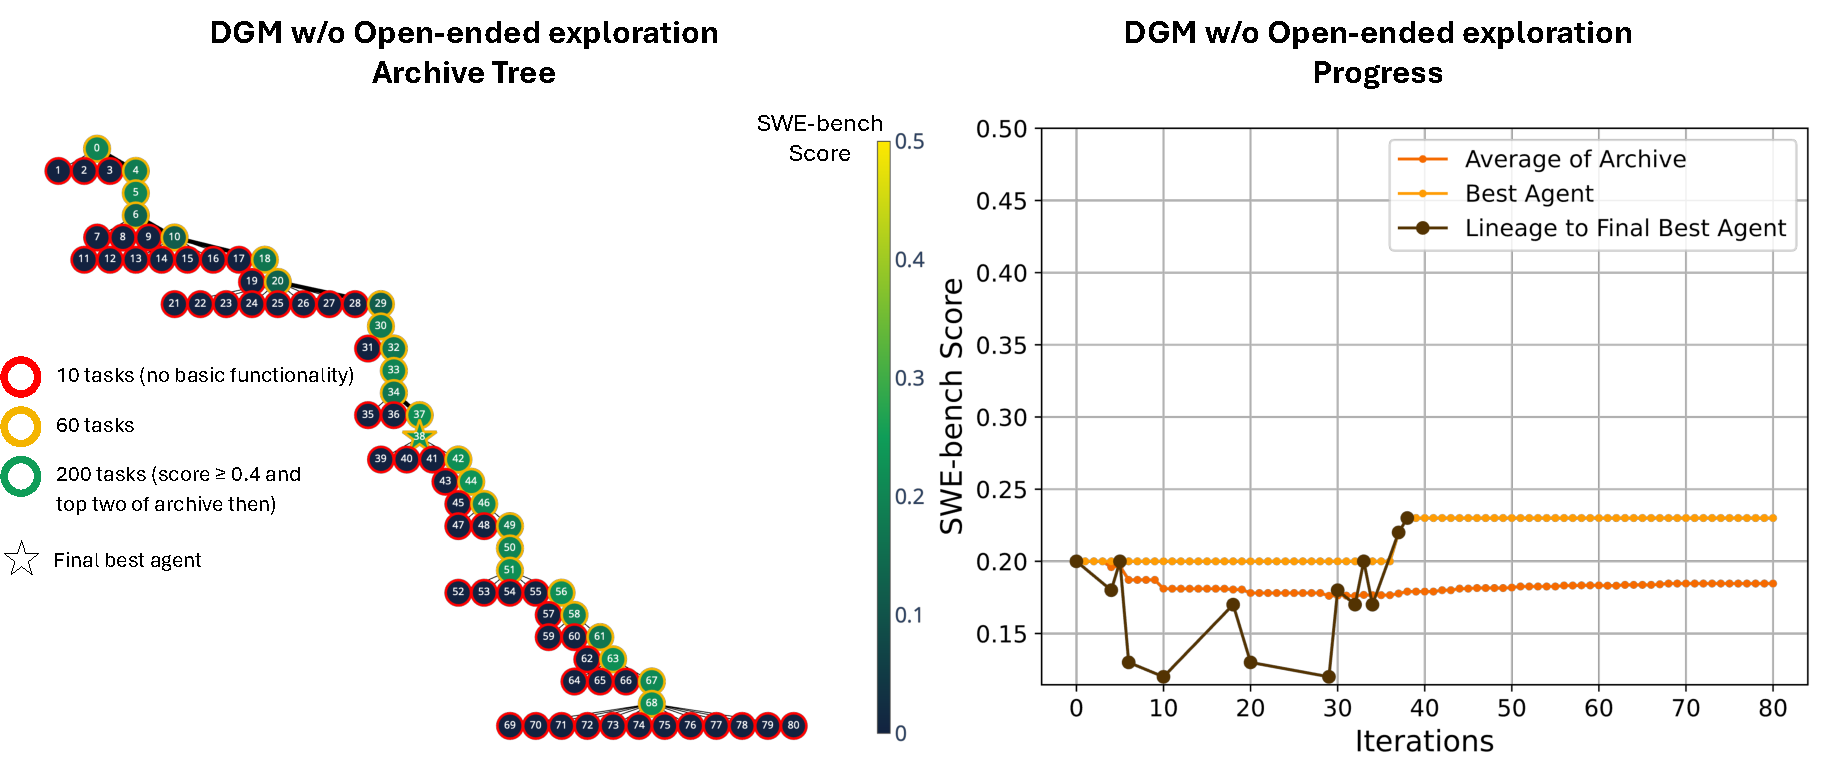
\includegraphics[width=0.95\textwidth]{figures/srcs/11_dgm_no_openended.pdf}
    \caption{\textbf{DGM without open-ended exploration.} Removing the archive, DGM w/o open-ended exploration always uses the most recent agent to self-modify and makes very little progress on SWE-bench. (Left) Archive of coding agents generated during the DGM w/o open-ended exploration run on SWE-bench. Each node represents a coding agent, with node 0 corresponding to the base agent. Node color indicates performance on SWE-bench (percentage of solved tasks), while border color reflects the number of tasks for which the agent was evaluated. Edges show which agents self-modified to produce the offsprings. (Right) Progress plot of the DGM w/o open-ended on SWE-bench. The orange line shows the average score of all agents possessing basic codebase-editing functionality. The light orange line tracks the best score achieved by any agent in the archive at each iteration. The dark line shows the lineage of the final best-discovered agent and its precursor nodes.}
    \label{fig:dgm-no-openended}
\end{figure}
